\documentclass[a4paper,oneside,12pt]{book}

%% Language %%%%%%%%%%%%%%%%%%%%%%%%%%%%%%%%%%%%%%%%%%%%%%%%%

\usepackage[USenglish]{babel} %francais, polish, spanish, ...
\usepackage[T1]{fontenc}
\usepackage[utf8x]{inputenc}
\usepackage{lmodern} %Type1-font for non-english texts and characters


%% Packages for Graphics & Figures %%%%%%%%%%%%%%%%%%%%%%%%%%

\usepackage{graphicx} %%For loading graphic files
\graphicspath{ {figures/} }

%% Other Packages %%%%%%%%%%%%%%%%%%%%%%%%%%%%%%%%%%%%%%%%%%%
\usepackage{caption}
\usepackage{listings}
\usepackage{xcolor}

\captionsetup[lstlisting]{font={small,tt}}

\definecolor{light-gray}{gray}{0.90}

\lstset{ %
	basicstyle=\ttfamily,
  backgroundcolor=\color{light-gray},   % choose the background color; you must add \usepackage{color} or \usepackage{xcolor}
  basicstyle=\scriptsize,        				% the size of the fonts that are used for the code
  breakatwhitespace=false,         			% sets if automatic breaks should only happen at whitespace
  breaklines=true,                 			% sets automatic line breaking
  captionpos=b,                    			% sets the caption-position to bottom
  %commentstyle=\color{mygreen},    		% comment style
  %deletekeywords={...},            		% if you want to delete keywords from the given language
  %escapeinside={\%*}{*)},          		% if you want to add LaTeX within your code
  %extendedchars=true,              		% lets you use non-ASCII characters; for 8-bits encodings only, does not work with UTF-8
  %frame=single,                    		% adds a frame around the code
  keepspaces=true,                 			% keeps spaces in text, useful for keeping indentation of code (possibly needs columns=flexible)
  %keywordstyle=\color{blue},      			% keyword style
  %language=Octave,                 		% the language of the code
  %morekeywords={*,...},            		% if you want to add more keywords to the set
  %numbers=left,                    		% where to put the line-numbers; possible values are (none, left, right)
  %numbersep=5pt,                   		% how far the line-numbers are from the code
  %numberstyle=\tiny\color{mygray}, 		% the style that is used for the line-numbers
  rulecolor=\color{black},         			% if not set, the frame-color may be changed on line-breaks within not-black text (e.g. comments (green here))
  showspaces=false,                			% show spaces everywhere adding particular underscores; it overrides 'showstringspaces'
  showstringspaces=false,          			% underline spaces within strings only
  showtabs=false,                  			% show tabs within strings adding particular underscores
  stepnumber=2,                    			% the step between two line-numbers. If it's 1, each line will be numbered
  stringstyle=\color{mymauve},     			% string literal style
  tabsize=2,                       			% sets default tabsize to 2 spaces
  %title=\lstname                   		% show the filename of files included with \lstinputlisting; also try caption instead of title
}

\usepackage{hyperref}
\hypersetup{
    colorlinks,
    citecolor=black,
    filecolor=black,
    linkcolor=black,
    urlcolor=black
}

%% A motivation environment %%%%%%%%%%%%%%%%%%%%%%%%%%%%%%%%%

\newenvironment{motivation}
{
   \vspace*{\stretch{1}}
}
{
   \vspace*{\stretch{3}}
   \clearpage
}

%%%%%%%%%%%%%%%%%%%%%%%%%%%%%%%%%%%%%%%%%%%%%%%%%%%%%%%%%%%%%
%% Options / Modifications
%%%%%%%%%%%%%%%%%%%%%%%%%%%%%%%%%%%%%%%%%%%%%%%%%%%%%%%%%%%%%

% Book's title and subtitle
\title{\Huge \textbf{An Introduction to Nmap} \\ \huge with a Focus on Information Gathering}
% Author
\author{\textsc{Ionuț Ambrosie}}
	%Military Technical Academy\\
	%Bucharest, Romania
	%}

%%%%%%%%%%%%%%%%%%%%%%%%%%%%%%%%%%%%%%%%%%%%%%%%%%%%%%%%%%%%%
%% THE DOCUMENT
%%%%%%%%%%%%%%%%%%%%%%%%%%%%%%%%%%%%%%%%%%%%%%%%%%%%%%%%%%%%%

\begin{document}

%% Frontmatter %%%%%%%%%%%%%%%%%%%%%%%%%%%%%%%%%%%%%%%%%%%%%%

\pagenumbering{roman}
\pagestyle{empty}

\maketitle

\begin{motivation}
During the information gathering phase of a penetration test, tools such as Nmap can be helpful in allowing one to discover what systems are alive on the target network and the software they're running. This information can later be used during the subsequent phases of the penetration test.

Since Nmap is a complex tool, someone who's just getting started might feel overwhelmed by the myriad of options. This guide tries to act as an introduction to Nmap for the purposes of host discovery, port scanning, version detection and OS fingerprinting.
\end{motivation}

\tableofcontents %Table of contents
\thispagestyle{empty}

%% Mainmatter %%%%%%%%%%%%%%%%%%%%%%%%%%%%%%%%%%%%%%%%%%%%%%%%%

\pagestyle{plain} %Now display headings: headings / fancy / ...
\clearpage
\pagenumbering{arabic}

\chapter{Introduction}
This guide assumes the reader has basic knowledge of the Internet Protocol suite (how TCP and UDP are related, how they use IP, what IP addresses and port numbers are and knowledge of the different TCP flags)\footnote{A good reference on the Internet protocol suite is TCP/IP Illustrated, Volume 1: The Protocols (2nd Edition) by Kevin R. Fall and W. Richard Stevens}.

\section{Setup}

In order to illustrate the techniques covered in this guide, we will be making use of the following setup (see Figure~\ref{fig:network_setup}): on our host operating system (vm.host) we have installed a hypervisor which runs a virtual machine with the Kali Linux distribution\footnote{Kali Linux is a Debian-derived GNU/Linux distribution designed for digital forensics and penetration testing use. The project's website is \url{https://www.kali.org/}} (vm.guest); the Kali Linux virtual machine's network connection is configured to run in NAT mode and has been assigned 192.168.60.128 as the IP address; the host operating system's IP address, as viewed from Kali Linux, is 192.168.60.2.

The two targets we're selected for this guide are:
\begin{description}
\item[scanme.nmap.org] is a service provided by the Nmap Security Scanner Project and Insecure.Org; before running the examples against this target, the reader is expected to read its rather brief terms of use by browsing to \url{http://scanme.nmap.org/}
\item[vm.host] is the host operating system in our setup
\end{description}

\begin{figure}[ht]
	\centering
	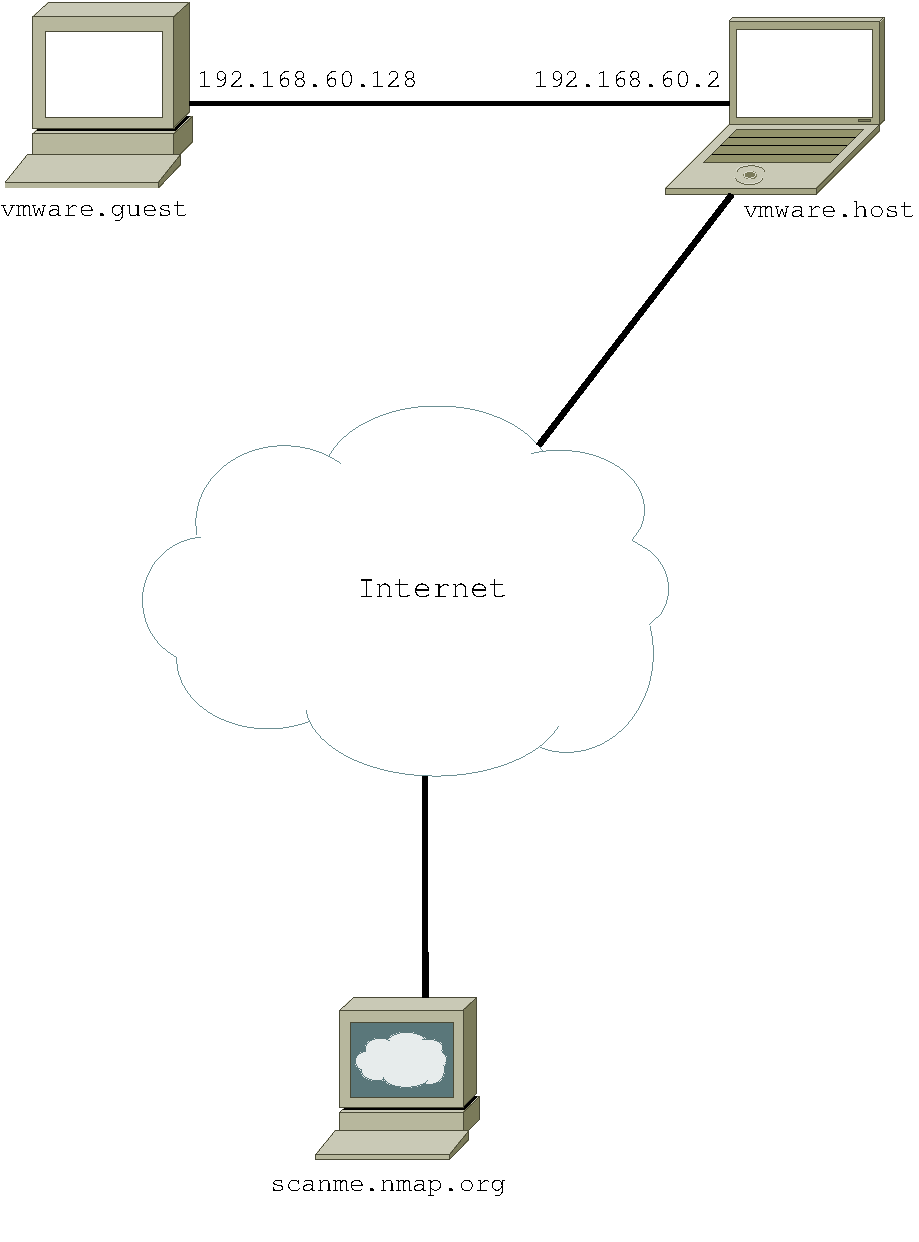
\includegraphics[scale=0.6]{setup}
	\caption{Our setup}
	\label{fig:network_setup}	
\end{figure}

\section{Nmap}

Nmap is an open source tool designed for network exploration and security auditing. Its output is composed of a list of scanned targets together with supplemental information on each, depending on the options used. Among that information is a table of ports which lists the port number, protocol, service name, and state. 

A port can be in either of the following states:
\begin{description}
\item[Open] means that an application on the target machine is listening for connections/packets on that port
\item[Closed] means ports have no application listening on them, though they could open up at any time
\item[Filtered] means that a firewall, filter, or other network obstacle is blocking the port so that Nmap cannot tell whether it is open or closed
\item[Unfiltered] means the ports are responsive to Nmap's probes, but Nmap cannot determine whether they are open or closed
\end{description}

Nmap reports the state combinations open|filtered and closed|filtered when it cannot determine which of the two states better describes a port.

The simplest way of running Nmap is by executing the \texttt{nmap target} command in your console. Here \texttt{target} can be an IP address (e.g. 192.168.60.2) or a hostname (e.g. vmware.host). In addition, Nmap supports CIDR-style addressing, multiple host specifications etc\footnote{Detailed information about specifying Nmap targets is available at \url{http://nmap.org/book/man-target-specification.html}}.

\begin{lstlisting}[title=A Nmap scan with no options]
root@kali:~# nmap vm.host

Starting Nmap 6.47 ( http://nmap.org ) at 2014-11-11 19:05 EET
Nmap scan report for vm.host (192.168.60.2)
Host is up (0.00071s latency).
Not shown: 999 closed ports
PORT   STATE SERVICE
53/tcp open  domain
MAC Address: 00:50:56:F3:FC:6F (VMware)

Nmap done: 1 IP address (1 host up) scanned in 1.24 seconds
\end{lstlisting}

By default, Nmap scans the most commonly used 1000 TCP ports on the target host. The \texttt{-p} option can be used for specifying which ports should be scanned (e.g. the argument \texttt{-pU:53,111,137,T:21-25,80,139,8080} instructs Nmap to scan UDP ports 53, 111 and 137, as well as TCP ports from 21 to 25, 80, 139 and 8080).

\chapter{Host Discovery}

Network scans usually begin by discovering which targets on the network are online and thus worth deeper investigation.

\section{No Port Scan (-sP)}

The -sP option instructs Nmap not to do a port scan after host discovery, and only print out the available hosts that respond to this scan. The default host discovery consists of an ICMP echo request, a TCP SYN segment to destination port 443, a TCP ACK segment to destination port 80, and an ICMP timestamp request. Also, for targets which are on a local ethernet network, an ARP scan is used.

\begin{lstlisting}[title=A Nmap scan using the No Port Scan option]
root@kali:~# nmap -sP scanme.nmap.org

Starting Nmap 6.47 ( http://nmap.org ) at 2014-11-05 15:25 EET
Nmap scan report for scanme.nmap.org (74.207.244.221)
Host is up (0.00029s latency).
Nmap done: 1 IP address (1 host up) scanned in 0.21 seconds
\end{lstlisting}

\section{ARP Ping (-PR)}

When scanning hosts in an ethernet LAN, the -PR option instructs Nmap to perform an ARP (Address Resolution Protocol) ping on the specified target. This type of discovery is much faster and more reliable than IP-based scans.

\begin{lstlisting}[title=A Nmap scan using the ARP Ping option]
root@kali:~# nmap -PR -sP vm.host

Starting Nmap 6.47 ( http://nmap.org ) at 2014-11-27 18:24 EET
Nmap scan report for vm.host (192.168.60.2)
Host is up (0.00075s latency).
MAC Address: 00:50:56:F3:FC:6F (VMware)
Nmap done: 1 IP address (1 host up) scanned in 0.14 seconds
\end{lstlisting}

\section{No Ping (-Pn)}

The -Pn option instructs Nmap to skip the default host discovery step and perform a port scan on the target hosts.

\begin{lstlisting}[title=A Nmap scan using the No Ping option]
root@kali:~# nmap -Pn scanme.nmap.org

Starting Nmap 6.47 ( http://nmap.org ) at 2014-11-27 18:46 EET
Nmap scan report for scanme.nmap.org (74.207.244.221)
Host is up (0.00082s latency).
Not shown: 992 closed ports
PORT      STATE    SERVICE
22/tcp    open     ssh
80/tcp    open     http
425/tcp   filtered icad-el
514/tcp   filtered shell
1047/tcp  filtered neod1
1147/tcp  filtered capioverlan
5987/tcp  filtered wbem-rmi
32779/tcp filtered sometimes-rpc21

Nmap done: 1 IP address (1 host up) scanned in 794.23 seconds
\end{lstlisting}

\chapter{Port Scanning}

After making sure the target system is alive, the natural next step is trying to identify the system's ports states. And while Nmap has evolved in functionality over the years, port scanning remains its core function.

When port scanning target hosts with Nmap, it's important to keep in mind only one method may be used at a time, except that, for example, a UDP scan (-sU) may be combined with any one of the TCP scan types.

As a memory aid, port scan type options are generally of the form -sC, where C is a prominent character in the scan name, usually the first. 

\section{SYN Scan (-sS)}

SYN scans are often referred to as half-open scanning because a full TCP connection is not opened.

A SYN scan works by sending a TCP segment with the SYN flag set (i.e. the first step in a TCP three-way handshake) and examining the response.

If the response consists of a TCP segment with the SYN and ACK flags set, then the port is listening (open). The port is also considered open if a TCP segment with SYN flag set (without the ACK flag set) is received in response. A response consisting of a TCP segment with the RST and ACK flag (reset) is indicative of a non-listener. And if no response is received after several retransmissions, the port is marked as filtered. Also, the port is also marked as filtered if an ICMP unreachable error (type 3, code 1, 2, 3, 9, 10, or 13) is received.

Also note that this is the default port scanning technique employed, provided that the user running Nmap has proper privileges to send and receive raw packets (e.g. Nmap is run as root).

\begin{lstlisting}[title=A sample Nmap scan using the SYN Scan option]
root@kali:~# nmap -sS -p20,80,514,9929 scanme.nmap.org

Starting Nmap 6.47 ( http://nmap.org ) at 2014-11-05 17:09 EET
Nmap scan report for scanme.nmap.org (74.207.244.221)
Host is up (0.00040s latency).
PORT     STATE    SERVICE
20/tcp   filtered ftp-data
80/tcp   open     http
514/tcp  filtered shell
9929/tcp filtered nping-echo

Nmap done: 1 IP address (1 host up) scanned in 1.62 seconds
\end{lstlisting}


\section{Connect Scan (-sT)}

A Connect scan consists of trying to establishing a connection with the target machine and port by issuing the connect system call. Because the system call completes connections to open target ports, rather than performing the half-open reset that a SYN scan does, this scanning technique takes longer and requires more packets to obtain the same information. Also, target machines are more likely to log the connection.

If the user running Nmap doesn't have the required privileges to send and receive raw packets (i.e. does not run Nmap as root), this will be the default scan type employed.

\begin{lstlisting}[title=A sample Nmap scan using the Connect Scan option]
root@kali:~# nmap -sT -p20,80,514,9929 scanme.nmap.org

Starting Nmap 6.47 ( http://nmap.org ) at 2014-11-05 17:17 EET
Nmap scan report for scanme.nmap.org (74.207.244.221)
Host is up (0.0035s latency).
PORT     STATE    SERVICE
20/tcp   filtered ftp-data
80/tcp   open     http
514/tcp  filtered shell
9929/tcp filtered nping-echo

Nmap done: 1 IP address (1 host up) scanned in 1.47 seconds
\end{lstlisting}

\section{NULL Scan (-sN), FIN Scan (-sF), Xmas Scan (-sX)}

These three scan types exploit a subtle loophole in the TCP RFC\footnote{RFC 793, \url{http://www.rfc-editor.org/rfc/rfc793.txt}} in order to differentiate between port states. 

When scanning systems compliant with the TCP RFC text (i.e. most Unix-based systems), any TCP segment not having the SYN, RST, or ACK flags set will result in receiving a TCP segment with the RST flag set, if the port is closed, or no response at all, if the port is open|filtered. If a TCP segment with the RST flag set is received, the port is considered closed, while no response means it is open|filtered. The port is marked filtered if an ICMP unreachable error (type 3, code 1, 2, 3, 9, 10, or 13) is received. 

While none of SYN, RST, or ACK flags should be set on the outgoing segments, any combination of the other three (FIN, PSH and URG) are O.K.

Thus, TCP NULL Scan (-sN) works by sending TCP segments without any flags set, TCP FIN Scan (-sF) works by sending TCP segments with just the FIN flag set, and TCP Xmas Scan (-sX) works by sending TCP segments with the FIN, PSH and URG flags set.

An important thing to note here is that some systems do not follow RFC 793 to the letter, the most prominent ones being Microsoft Windows and many Cisco devices. These systems send RST responses to probes employed by these scan types, regardless of whether the port is open or not. This causes all of the ports to be labeled as closed.

\begin{lstlisting}[title=A sample Nmap scan using the NULL Scan option]
root@kali:~# nmap -sN -p20,80,514,9929 scanme.nmap.org

Starting Nmap 6.47 ( http://nmap.org ) at 2014-11-10 17:08 EET
Nmap scan report for scanme.nmap.org (74.207.244.221)
Host is up (0.00031s latency).
PORT     STATE         SERVICE
20/tcp   open|filtered ftp-data
80/tcp   open|filtered http
514/tcp  open|filtered shell
9929/tcp open|filtered nping-echo

Nmap done: 1 IP address (1 host up) scanned in 1.64 seconds
\end{lstlisting}

\begin{lstlisting}[title=A sample Nmap scan using the FIN Scan option]
root@kali:~# nmap -sF -p20,80,514,9929 scanme.nmap.org

Starting Nmap 6.47 ( http://nmap.org ) at 2014-11-10 17:09 EET
Nmap scan report for scanme.nmap.org (74.207.244.221)
Host is up (0.00030s latency).
PORT     STATE         SERVICE
20/tcp   open|filtered ftp-data
80/tcp   open|filtered http
514/tcp  open|filtered shell
9929/tcp open|filtered nping-echo

Nmap done: 1 IP address (1 host up) scanned in 1.65 seconds
\end{lstlisting}

\begin{lstlisting}[title=A sample Nmap scan using the Xmas Scan option]
root@kali:~# nmap -sX -p20,80,514,9929 scanme.nmap.org

Starting Nmap 6.47 ( http://nmap.org ) at 2014-11-10 17:10 EET
Nmap scan report for scanme.nmap.org (74.207.244.221)
Host is up (0.00037s latency).
PORT     STATE         SERVICE
20/tcp   open|filtered ftp-data
80/tcp   open|filtered http
514/tcp  open|filtered shell
9929/tcp open|filtered nping-echo

Nmap done: 1 IP address (1 host up) scanned in 1.62 seconds
\end{lstlisting}

\section{ACK Scan (-sA)}

This scan method is used to map out firewall rulesets (i.e. determining whether they are stateful or not and which ports are filtered). By default, the ACK scan probe has only the ACK flag set. 

When scanning unfiltered systems, open and closed ports will both return a RST segment. Nmap then labels them as unfiltered, meaning that they are reachable by the ACK segment, but whether they are open or closed is undetermined. Ports that don't respond, or send certain ICMP error messages back (type 3, code 1, 2, 3, 9, 10, or 13), are labeled as filtered.

\begin{lstlisting}[title=A sample Nmap scan using the ACK Scan option]
root@kali:~# nmap -sA -p20,80,514,9929 scanme.nmap.org

Starting Nmap 6.47 ( http://nmap.org ) at 2014-11-10 17:52 EET
Nmap scan report for scanme.nmap.org (74.207.244.221)
Host is up (0.00030s latency).
PORT     STATE      SERVICE
20/tcp   unfiltered ftp-data
80/tcp   unfiltered http
514/tcp  unfiltered shell
9929/tcp unfiltered nping-echo

Nmap done: 1 IP address (1 host up) scanned in 0.28 seconds
\end{lstlisting}

\section{IDLE Scan (-sI)}

This is an advanced scan method which allows for a truly blind TCP port scan of the target, meaning no packets are sent to the target from your real IP address.

This is made possible by employing a clever side-channel attack\footnote{You can read more about how IDLE scan works at \url{http://nmap.org/book/idlescan.html}} which allows for the scan to be bounced off a dumb ``zombie host''. As such, intrusion detection systems will report the innocent zombie as the attacker.

Also, it's important to note that the port listing will shows open ports from the perspective of the zombie host. Thus, you can try scanning a target using various zombies that you think might be trusted (via router/packet filter rules).

An important note with regard to IDLE scans is that often times it is desirable to use it in conjunction with the No Ping option (-Pn), so to prevent pings from the real scanning machine.

One should also consider changing the default source port used for the zombie machine. This can be done by adding a colon, followed by a port number, when specifying the zombie host. By default, Nmap will use TCP 80 as the zombie source port.

\begin{lstlisting}[title=A sample Nmap scan using the IDLE Scan option]
root@kali:~# nmap -Pn -sI vm.host:443 -p80 scanme.nmap.org

Starting Nmap 6.47 ( http://nmap.org ) at 2014-11-12 15:31 EET
Idle scan using zombie vm.host (192.168.60.2:443); Class: Incremental
Nmap scan report for scanme.nmap.org (74.207.244.221)
Host is up (0.19s latency).
PORT   STATE SERVICE
80/tcp open  http

Nmap done: 1 IP address (1 host up) scanned in 70.11 seconds
80/tcp open  http

Nmap done: 1 IP address (1 host up) scanned in 41.05 seconds
\end{lstlisting}

\section{UDP Scan (-sU)}

Although the most popular services on the Internet run over the TCP protocol, there exist UDP services which are widely deployed, e.g. DNS, SNMP, and DHCP (registered ports 53, 161/162, and 67/68). As such, Nmap offers the option of a UDP scan with the -sU option. UDP scanning can be combined with a TCP scan type, such as SYN scan (-sS), to check both protocols during the same run.

UDP scan works by sending a UDP packet to every targeted port. If an ICMP port unreachable error (type 3, code 3) is returned, the port is labeled as closed. Other ICMP unreachable errors (type 3, codes 1, 2, 9, 10, or 13) mark the port as filtered. Occasionally, a service will respond with a UDP packet, proving that it is open. If no response is received after a number of retransmissions, the port is classified as open|filtered.

\begin{lstlisting}[title=A sample Nmap scan using the UDP Scan option]
root@kali:~# nmap -sU -pU:53,161,162,67,68 scanme.nmap.org

Starting Nmap 6.47 ( http://nmap.org ) at 2014-11-10 17:56 EET
Nmap scan report for scanme.nmap.org (74.207.244.221)
Host is up (0.00028s latency).
PORT    STATE         SERVICE
53/udp  open|filtered domain
67/udp  open|filtered dhcps
68/udp  open|filtered dhcpc
161/udp open|filtered snmp
162/udp open|filtered snmptrap

Nmap done: 1 IP address (1 host up) scanned in 1.49 seconds
\end{lstlisting}

\chapter{Version Detection}

While it is useful to know whether certain ports on a remote machine are open or closed, you sometimes want to know which email, DNS and HTTP servers are running and their respective versions. This might be extremely useful, because having an accurate version number helps dramatically in determining which exploits a server is vulnerable to. Thus, Nmap provides the -sV option for enabling version detection.

Version detection works by interrogating those TCP or UDP ports flagged as open or open|filtered during the port scanning phase\footnote{A detailed resource on using Nmap for the purposes of OS detection is \url{http://nmap.org/book/vscan.html}}, with the purpose of identifying the software version that is actually running on those particular ports.

It's also worth mentioning that one of the key components of version detection is the nmap-service-probes database which contains probes for querying various services and match expressions to recognize and parse responses.

\begin{lstlisting}[title=A sample Nmap scan using the Version Detection option]
root@kali:~# nmap -sV -p20,80,514,9929 scanme.nmap.org

Starting Nmap 6.47 ( http://nmap.org ) at 2014-11-10 16:28 EET
Nmap scan report for scanme.nmap.org (74.207.244.221)
Host is up (0.00068s latency).
PORT     STATE    SERVICE    VERSION
20/tcp   filtered ftp-data
80/tcp   open     http       Apache httpd 2.2.14 ((Ubuntu))
514/tcp  filtered shell
9929/tcp filtered nping-echo

Service detection performed. Please report any incorrect results at http://nmap.org/submit/ .
Nmap done: 1 IP address (1 host up) scanned in 10.17 seconds
\end{lstlisting}

\chapter{OS Detection}

Another useful feature provided by Nmap is remote OS detection using TCP/IP stack fingerprinting.

OS detection works by sending a series of TCP and UDP packets to the remote host and examining the responses. After performing some tests, Nmap then compares the results to its nmap-os-db database and prints out the OS details, if there is a match.

While the inner workings of OS detection are quite complex, it is one of the easiest features to use\footnote{A more detailed resource on using Nmap for the purposes of OS detection is \url{http://nmap.org/book/osdetect.html}
}.

OS detection is enabled by providing the -O parameter when starting Nmap. Additionally, one can increase the verbosity level with -v for even more OS-related details.

\begin{lstlisting}[title=A sample Nmap scan using the OS detection option]
root@kali:~# nmap -O scanme.nmap.org

Starting Nmap 6.47 ( http://nmap.org ) at 2014-11-10 16:37 EET
Nmap scan report for scanme.nmap.org (74.207.244.221)
Host is up (0.28s latency).
Not shown: 996 closed ports
PORT     STATE    SERVICE
22/tcp   open     ssh
80/tcp   open     http
514/tcp  filtered shell
9929/tcp open     nping-echo
Device type: general purpose|storage-misc|VoIP phone
Running (JUST GUESSING): Linux 2.4.X|3.X (98%), Microsoft Windows 7|XP (96%), BlueArc embedded (91%), Pirelli embedded (88%)
OS CPE: cpe:/o:linux:linux_kernel:2.4 cpe:/o:linux:linux_kernel:3 cpe:/o:microsoft:windows_7:::enterprise cpe:/o:microsoft:windows_xp::sp3 cpe:/h:bluearc:titan_2100 cpe:/h:pirelli:dp-10
Aggressive OS guesses: DD-WRT v24-sp2 (Linux 2.4.37) (98%), Linux 3.2 (98%), Microsoft Windows 7 Enterprise (96%), Microsoft Windows XP SP3 (96%), BlueArc Titan 2100 NAS device (91%), Pirelli DP-10 VoIP phone (88%)
No exact OS matches for host (test conditions non-ideal).

OS detection performed. Please report any incorrect results at http://nmap.org/submit/ .
Nmap done: 1 IP address (1 host up) scanned in 152.86 seconds
\end{lstlisting}

\chapter{Conclusions}

As mentioned in the begining of this document, Nmap is a complex tool. As such, this guide tried to act as an introduction to some of its most common usage scenarios. It is the author's hope that his efforts weren't in vain.

The next step, should one feel like furthering his Nmap understanding, should consist of consulting the tool's man page. This can achieved by issuing the \texttt{man nmap} shell command. Another option is purchasing and reading the book ``Nmap Network Scanning'', written by Nmap's original author, Gordon ``Fyodor'' Lyon~\footnote{About half of the book's content is available for free at \url{http://nmap.org/book/toc.html}}.

\end{document}

